\documentclass[11pt]{article}

%opening
\title{TMR: Detecting Structure in Graphical Data}
\author{Lawrence Tray \and Ioannis Kontoyiannis}

%packages
\usepackage[margin=0.6in]{geometry}
\usepackage{graphicx}
\usepackage{amsmath}
\usepackage{amssymb}
\usepackage{hyperref}
\usepackage{caption}
\usepackage{subcaption}
\usepackage{mathtools}
\usepackage{parskip}
\usepackage{fancyvrb}
\usepackage{bbm}
\usepackage{algorithm}% http://ctan.org/pkg/algorithm
\usepackage{algpseudocode}% http://ctan.org/pkg/algorithmicx
\usepackage{multicol}
\usepackage{titling}


%bibliography
\usepackage[backend=bibtex]{biblatex}
\addbibresource{interim-sources.bib}

%title
\setlength{\droptitle}{-4em}   % This is your set screw

%package setup
\graphicspath{{./img/}}
\DeclareMathOperator*{\argmax}{arg\,max}
\DeclareMathOperator*{\argmin}{arg\,min}

%custom commands
\newcommand{\dft}{\mathcal{F}}
\newcommand{\idft}{\mathcal{F}^{-1}}
\newcommand{\Xcal}{\mathcal{X}}
\newcommand{\Dcal}{\mathcal{D}}
\newcommand{\cmplx}{\mathbb{C}}
\newcommand{\E}{\mathbb{E}}
\newcommand{\Gaussian}{\mathcal{N}}
\newcommand{\Gcal}{\mathcal{G}}
\newcommand{\Vcal}{\mathcal{V}}
\newcommand{\Ecal}{\mathcal{E}}
\newcommand{\pbold}{\boldsymbol{p}}
\newcommand{\sigmabold}{\boldsymbol{\sigma}}
\newcommand{\lik}{\mathcal{L}}
\newcommand{\kl}{\mathcal{D}}
\newcommand{\Integers}{\mathbb{Z}}
\newcommand{\SBM}{\textrm{SBM}}
\newcommand{\iid}{\stackrel{iid}{\sim}}
\newcommand{\one}{\mathbbm{1}}
\newcommand{\prob}{\mathbbm{P}}
\newcommand{\figwidth}{0.7\linewidth}


% definition
\newtheorem{definition}{Definition}[section]
\newtheorem{theorem}{Theorem}[section]
\newtheorem{corollary}{Corollary}[theorem]
\newtheorem{lemma}[theorem]{Lemma}


\begin{document}

\maketitle

\begin{abstract}
We produce vast quantities of graphical data every day and yet the techniques used to analyse their structure are still in their infancy. We begin with the definition of the Stochastic Block Model (SBM) widely used in academia and develop a theorem to verify structure in a labelled graph through a hypothesis test. We explore the results of applying this theorem to Facebook friendship egonets and find that gender does indeed influence how friendships form on Facebook. Nevertheless, this binary yes-no result is unsatisfactory.

To rank order vertex labels by importance we instead approach the problem from the opposite direction: given a graph we detect the partitions that are in some sense typical and then develop a classifier to map from vertex features to partition. The classifier then implicitly rank orders the input features automatically. Nevertheless, work must still be done to refine this classifier and tie it back to the rigorous hypothesis testing framework already developed.
\end{abstract}

\begin{multicols*}{2}

\section{Introduction}

There is a wealth of graphical data in the world with more produced every second; social networks, website hyperlinks and academic collaboration are just some examples. Many algorithms are used to analyse this data. Nevertheless, the same principled hypothesis testing framework we have for querying classical data is less well-developed for graphical data. Do my friends vote the same way I do or do researchers collaborate with those of the same gender? We want to answer these questions and not only that, we wish to report our confidence in the answers. To that end we seek to expand the hypothesis testing framework to graphs.

\section{The Stochastic Block Model}

The most popular graphical model in academia is called the Stochastic Block Model (SBM). We use a definition adapted from Abbe \cite{Abbe}.

\begin{definition}
	\label{defn:sbm}
	Let $n \in \Integers^+$ be the number of vertices and $k \in \Integers^+$ be the number of communities. We define the vector $p = [p_1, p_2 \dots p_k]^T$ to be the prior on the k-communities. Each vertex $v \in \Vcal = \{1, 2 \dots n\}$ has a community label $X_v \in \{1, 2 \dots n\}$. Let $W$ be a symmetric $k \times k$ matrix with entries in $[0,1]$ called the connectivity matrix. The pair $(X, \Gcal) \sim \textrm{SBM}(n, p, W)$ if X is an $n \times 1$ vector with each component independently drawn from the community prior $X_v \sim p$ and $\Gcal$ is an $n$-vertex graph where each vertex-pair $(i, j)$ is connected with probability $\prob(i \leftrightarrow j) = W_{X_i, X_j}$ independently of other edges. Lastly, we define the community sets as $\Omega_i = \Omega_i(X) \coloneqq \{v \in \Vcal : X_v = i\}$ which contains all vertices belonging to community $i$.
\end{definition}

\section{Verifying Structure}
\subsection{Theory}

Armed with definition \ref{defn:sbm} we tackle the simplest problem in structure verification. Given an undirected graph $\Gcal$ and vertex-labels $X$ such that $(X, \Gcal) \sim \textrm{SBM}(n, p, W)$, we wish to determine whether two communities $a$ and $b$ connect differently. Put formally, this is a hypothesis test on the parameters of $W$. There are three parameters we would wish to test: $W_{aa}, W_{ab}$ and $W_{bb}$ (note that for an undirected graph $W = W^T$ necessarily so $W_{ab} = W_{ba}$). To do this we can perform three-pairwise hypothesis tests. Here we test $W_{\alpha}$ against $W_{\beta}$ where $\alpha$ and $\beta$ are unique index pairs in $\{(a,a), (a, b), (b,b)\}$. Therefore, each hypothesis test can be formulated as below:
%
\begin{equation}
\begin{aligned}
	H_0:& \quad W_{\alpha} = W_{\beta} \\
	H_1:& \quad W_{\alpha} \neq W_{\beta}
\end{aligned}
\end{equation}
%
We formulate this as a likelihood ratio test. Letting $\lik(D | H)$ denote the likelihood of observing the data $D = (X, \Gcal)$ under hypothesis $H$. Therefore, the test statistic is given by:
%
\begin{equation}
	t_n \coloneqq \log \frac{\lik(D | H_1)}{\lik(D | H_0)}
	\label{eqn:test-statistic-start}
\end{equation}
%
At this point it helps to introduce some more notation. We define the number of vertices in community $i$ by $n_i \coloneqq |\Omega_i(X)|$. Furthermore, we use $E_{ij} = E_{ij}(X, \Gcal)$ to denote the number of realised edges between communities $i$ and $j$ (in generality $i$ may be equal to $j$) and similarly define $M_{ij} = M_{ij}(X)$ as the maximum number of possible edges between communities $i$ and $j$. This is computed simply as follows:
%
\begin{equation}
	M_{ij} = M_{ij} (X) = \begin{cases}
		n_i n_j &\text{for } i \neq j \\
		\frac{1}{2}n_i (n_i - 1) &\text{for } i = j
	\end{cases}
\end{equation}
%
With this new notation, the likelihood function can be written explicitly:
%
\begin{align}
\lik(D | H) &= \prob(X| p) \cdot \prob(\Gcal | W, X) \nonumber \\
&= \prob(X | p) \prod_{i=1}^{k} \prod_{j=i}^{k} \prob(E_{ij} | W, X) \nonumber \\
&= \prob(X | p) \prod_{i=1}^{k} \prod_{j=i}^{k} W_{ij} ^ {E_{ij}} \left( 1 - W_{ij} \right) ^ {(M_{ij} - E_{ij})}
\label{eqn:likelihood-verbose}
\end{align}
%
By inspecting equation \ref{eqn:likelihood-verbose} we see that only terms involving $W_{\alpha}$ and $W_{\beta}$ are going to differ under the two hypotheses $H_0$ and $H_1$; the rest of the terms will cancel in our calculation of the test-statistic $t_n$. Therefore, we can rewrite the likelihood as follows:
%
\begin{equation}
	\lik (D | H) \propto f (W_\alpha, E_\alpha, M_\alpha) \cdot f (W_\beta, E_\beta, M_\beta)
\end{equation} 
\begin{equation}
	\textrm{where } f (w, e, m) \coloneqq w^e \cdot (1-w)^{(m - e)}
	\label{eqn:f-defn}
\end{equation}
%
We note that $f(w, e, m)$ is simply the probability of observing a specific sequence of $e$ successes in $m$ independent Bernoulli trials with parameter $w$. Its maximiser with respect to the first argument is easily computed through partial differentiation giving:
%
\begin{equation}
	\argmax_w f(w, e, m) = \hat{w} = e / m
	\label{eqn:f-maximiser}
\end{equation}
%
Furthermore, we spot the following property $f(w, e_1, m_1) \cdot f(w, e_2, m_2) = f(w, e_1 + e_2, m_1 + m_2)$ or in other words, the function $f$ is linear in its second and third arguments given the same first argument. As such we can manipulate equation \ref{eqn:test-statistic-start} greatly to give:
%
\begin{align}
	t_n &= \log \frac
	{
		\max_{W_{\alpha} \neq W_{\beta}}(f (W_\alpha, E_\alpha, M_\alpha) \cdot f (W_\beta, E_\beta, M_\beta))
	}
	{
		\max_{W_\alpha = W_\beta} (f (W_\alpha, E_\alpha, M_\alpha) \cdot f (W_\beta, E_\beta, M_\beta))
	} \nonumber \\
	&= \log \frac{
		\max_p f(p, E_\alpha, M_\alpha) \cdot \max_q f(q, E_\alpha, M_\alpha)
	}{
		\max_r f(r, E_\alpha + E_\beta, M_\alpha + M_\beta)
	} \nonumber \\
	&= \log \frac{f(\hat{p}, E_\alpha, M_\alpha)}{f(\hat{r}, E_\alpha, M_\alpha)} + \log \frac{f(\hat{q}, E_\beta, M_\beta)}{f(\hat{r}, E_\beta, M_\beta)}
\end{align}
%
Where $\hat{p} \coloneqq E_\alpha / M_\alpha$, $\hat{q} \coloneqq E_\beta / M_\beta$ and $\hat{r} \coloneqq (E_\alpha + E_\beta) / (M_\alpha + M_\beta)$. These are essentially maximum-likelihood estimates of parameters of $W$ constrained by the corresponding hypothesis. Note that the max-likelihood estimate of $W_\alpha$ under $H_1$ is denoted by the symbol $\hat{p}$ and should not be confused with the community prior $p$ though context will make the distinction apparent. We now state lemma \ref{lem:kl-div}.

\begin{lemma}[KL divergence]
	With $f$ defined as in equation \ref{eqn:f-defn}, $0 \leq e \leq m$ and $r \in [0, 1]$ it holds that:
	%
	\begin{equation*}
		\log \frac{f(e/m, e, m)}{f(r, e, m)} = m \cdot \kl \left( \textrm{Bern}(e/m) || \textrm{Bern}(r) \right)
	\end{equation*}

	where $\kl(g || h)$ is the Kullback-Leibler divergence between two probability mass functions $g, h: \Xcal \mapsto [0, 1]$. $\kl$ is defined in discrete space as $\kl(g || h) \coloneqq \sum_{x \in \Xcal} g(x) \log \frac{g(x)}{h(x)}$ and $\textrm{Bern(p)}$ denotes the Bernoulli p.m.f with parameter $p$.
	\label{lem:kl-div}
\end{lemma}

Proving lemma \ref{lem:kl-div} is simply a case of algebraic manipulation and is omitted here. However, this allows us to simplify the test-statistic into a form that is easier to compute (equation \ref{eqn:test-stat-compute-form}). However, we must simplify further still using lemma \ref{lem:kl-approx-chi}.
%
\begin{equation}
	\begin{aligned}
	t_n = &M_\alpha \kl\left( \textrm{Bern}(\hat{p}) || \textrm{Bern}(\hat{r})\right) \\
	&+ M_\beta \kl\left( \textrm{Bern}(\hat{q}) || \textrm{Bern}(\hat{r})\right)
	\end{aligned}
	\label{eqn:test-stat-compute-form}
\end{equation}
%
\begin{lemma}[$\chi^2$ approximation]
	\label{lem:kl-approx-chi}
	For $g(x) \approx h(x)$ then $\kl(g || h) \approx \frac{1}{2} \chi^2(g || h)$ where $\chi^2$ is the chi-squared distance between two distributions defined as $\chi^2(g || h) \coloneqq \sum_{x \in \Xcal} \frac{(g(x)-h(x))^2}{h(x)}$ 
\end{lemma}

The proof requires defining $\delta(x) \coloneqq g(x) - h(x)$ and taking a Taylor expansion of $\log (1 + \delta / h)$ - omitted for bervity. The chi-squared distance between two Bernoullis $g = Bern(p)$ and $h = Bern(q)$ has a very simple form:
%
\begin{equation}
\chi^2(\textrm{Bern}(p) || \textrm{Bern}(q)) = \left( \frac{p-q}{\sqrt{q(1-q)}} \right)^2
\end{equation}
%
We can apply these results to equation \ref{eqn:test-stat-compute-form} to obtain an approximate expression for $t_n$ under the null. Under $H_0$ and for large $n$, the estimates $\hat{p}$, $\hat{q}$ and $\hat{r}$ are all close meaning Lemma \ref{lem:kl-approx-chi} is applicable. This gives:
%
\begin{align}
	t_n &\approx \frac{1}{2 \hat{r}(1 - \hat{r})} \left( 
	M_\alpha \left(\hat{p} - \hat{r}\right)^2 +
	M_\beta \left(\hat{q} - \hat{r} \right)^2 
	\right) \nonumber \\
	&= \frac{1}{2} \left( \frac{\hat{p} - \hat{q}}{\sqrt{\hat{r}(1- \hat{r})(1/M_\alpha + 1/M_\beta)}} \right)^2
	= \frac{1}{2} z_n^2
\end{align}
%
Through application of the Central Limit Theorem (CLT) and Slutsky's Theorem it can be shown that as $n \rightarrow \infty$ under the null, the term in brackets on the final line is distributed like a standard Gaussian $z_n \sim \Gaussian(0,1)$. The proof is long-winded and therefore omitted from this short report. The result leads to theorem \ref{theorem:hyp-test-sbm-chi}.

\begin{theorem}[$\chi^2$ test]
	For $(X, \Gcal) \sim \textrm{SBM}(n, p, W)$, given the realised graph and class labels $(X, \Gcal)$ we can perform a hypothesis test on entries $W_\alpha$ and $W_\beta$ of the connectivity matrix $W$.
	%
	\begin{align*}
	H_0:& \quad W_{\alpha} = W_{\beta} \\
	H_1:& \quad W_{\alpha} \neq W_{\beta}
	\end{align*}
	If the log-likelihood ratio test statistic $t_n$ is computed as in equation \ref{eqn:test-stat-compute-form}, then as the number of vertices $n \rightarrow \infty, t_n \sim \frac{1}{2} \chi^2_1$ under the null $H_0$. Therefore, we reject $H_0$ at the $100(\zeta)\%$ confidence level if and only if $2t_n \geq \psi^{-1}(\zeta)$, where $\psi^{-1}$ is the $\chi^2_1$ inverse cdf satisfying $\prob(Y \leq \psi^{-1}(\zeta)) = \zeta$ given $Y \sim \chi^2_1$.
	
	\label{theorem:hyp-test-sbm-chi}
\end{theorem}

Indeed, a corollary is the hypothesis test possible by comparing $z_n$ to a standard Gaussian.

\subsection{Early results}

We seek to apply theorem \ref{theorem:hyp-test-sbm-chi} to real-world graphical datasets. We start by analysing social network graphs. The Stanford Network Analysis Project (SNAP) \cite{snapnets} offers a wealth of Facebook egonets. An egonet is simply a graph where all vertices (in this case Facebook users) are connected to one central node (the ego-node). The data consists of the undirected set of edges $\Gcal$ indicating whether any two vertices are connected (friends on Facebook) and matrix $F$ containing binary feature flags for each vertex. Example feature flags are given below: \\

\begin{center}
\begin{minipage}{8cm}
\begin{Verbatim}[fontsize=\small, frame=single, label={\fbox{Example anonymised feature flags}}]
75 first_name;anonymized feature 75
76 first_name;anonymized feature 76
77 gender;anonymized feature 77
78 gender;anonymized feature 78
79 hometown;id;anonymized feature 79
\end{Verbatim}
\end{minipage}
\end{center}


Each feature is given an anonymised signature to avoid disclosing personally identifiable information. If we have a total of $f$ features and $n$ vertices, then the feature matrix $F$ would have shape $n \times f$ where each row is the feature vector for the corresponding vertex. Each feature is encoded with a binary flag such that $F_{ij} \in \{0, 1\}$ indicating feature turned off and on respectively.

We perform a hypothesis test in the manner described by theorem \ref{theorem:hyp-test-sbm-chi} to determine whether gender influences how friends connect on Facebook. We choose to analyse SNAP egonet with id 0 (the id of the egonet is the id of the single egonode). The egonet is plotted on figure \ref{fig:ego-0-by-gender} with nodes coloured by gender. We use the Python package NetworkX \cite{networkx} for its graph visualisation tools. Indeed, we will discuss layout algorithms later as for now we focus on the hypothesis test.
%
\begin{figure}[H]
	\centering
	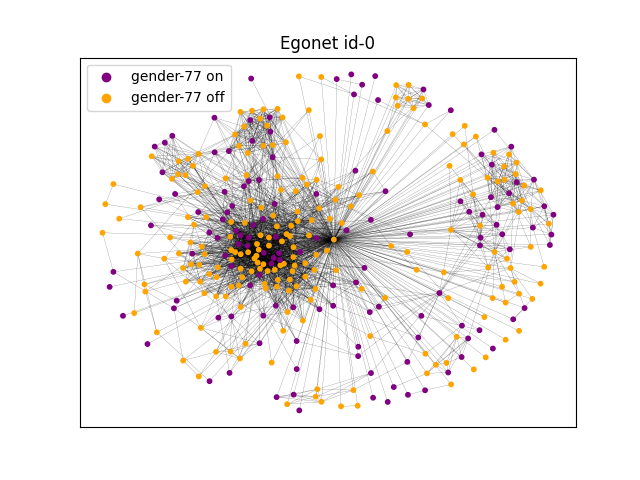
\includegraphics[width=\figwidth]{ego-0-by-gender.png}
	\caption{Egonet 0 with nodes coloured by gender}
	\label{fig:ego-0-by-gender}
\end{figure}

We use an SBM model with $k=2$ communities (1: gender-77 on and 2: gender-77 off) to model the egonet and perform a three-way hypothesis test on the parameters of the connectivity Matrix $W$.
%
\begin{equation}
	W = \begin{bmatrix}
		p_1 & q \\
		q & p_2
	\end{bmatrix}
\end{equation}
%
Therefore, $p_1$ is the probability that two vertices of gender-77 are connected, $q$ is the crossover probability and $p_2$ is the connection probability within the gender-78 community
\footnote{Strictly speaking this is the not gender-77 community as there are a handful of vertices that do not disclose their gender to Facebook or do not fall into this binary}
. The results of the hypothesis tests are given in table \ref{tab:egonet-0-hyp-tests} alongside p-values (we choose a 95\% significance level to reject the null). However, in some cases the test statistics were so extreme that the p-value saturated to 0.
%
\begin{table}[H]
	\centering
	\begin{tabular}{c c c c c}
		$n_1$                & $n_2$                & $\hat{p_1}$ & $\hat{q}$ & $\hat{p_2}$       \\ \hline
		130 & 218 & $8.13 \times 10^{-2}$ & $7.66 \times 10^{-2}$ & $10.6 \times 10^{-2}$
	\end{tabular}
	\caption{Egonet-0 properties and parameter estimates}
	\label{tab:egonet-0-props}
\end{table}
%
\begin{table}[H]
	\centering
	\begin{tabular}{cccccc}
		Test & $H_0$                & $H_1$                & p-value & $H_0$ rejected       \\ \hline
		1    & $p_1 = q$            & $p_1 \neq q$         & 0.158 &  No                \\
		2    & $p_1 = p_2$ & $p_1 \neq p_2$ & 0.000 & Yes \\
		3    & $q = p_2$ & $q \neq p_2$ &  0.000 & Yes
	\end{tabular}
	\caption{Egonet-0 hypothesis test results}
	\label{tab:egonet-0-hyp-tests}
\end{table}

Test 2 rejecting the null gives evidence that gender-78 people (community 2) have on average more same-gender friends than 77-ers have ($\hat{p}_2 > \hat{p}_1$ in table \ref{tab:egonet-0-props}). The rejection of the null in test 3 gives evidence that gender-78 treat gender-77 people differently to their own gender. Indeed, a gender-78 person is more likely to be friends with a fellow 78-er than with a 77-er ($\hat{p}_2 > \hat{q}$).

However, we do not reject the null in test 1 as there is insufficient evidence to claim the reverse (that 77-ers tend to stay away from 78-ers). Nevertheless, these are results on a single egonet so can hardly be generalised to society as a whole.

However, the exercise has highlighted some interesting points. The hypothesis test framework does not quantify the magnitude of the difference just whether or not a difference exists. Furthermore, The method relies on the analyst to specify the features of interest so results may be misleading if third variables are missing from the analysis.

To address these shortcomings we instead approach the problem from a different angle. For now we have been given a graph with fully labelled vertices and ask if a given feature affects the structure. Instead, we could take a graph and partition first (without using feature information) and then ask which features explain the partition. For that we need a way of detecting structure.

\section{Detecting Structure}
\subsection{Weak recovery}

Community detection is the problem of recovering the communities from the graph $\Gcal$. There are 4 recovery regimes (plus the trivial no recovery), as defined by Abbe \cite{Abbe}. We choose to focus on weak recovery as it is the least strict of all. Therefore, there are very few constraints on the SBM parameters and the theory can be applied to a wide range of graphs. A statement of weak recovery is given in definition \ref{defn:weak-recovery} (adapated from \cite{Abbe}).

\begin{definition}[Weak recovery]
	\label{defn:weak-recovery}
	weak recovery is solved for a graph  $(X, \Gcal) \sim \textrm{SBM}(n, p, W)$ if there exists $\epsilon > 0$, a certain choice of indices $i, j \in \{1, 2 \dots k\}$ and an algorithm that takes as input $\Gcal$ and outputs a partition of the vertex set $\Vcal$ into two distinct sets $S$ and $S^C$ (detected communities 1 and 2 respectively) such that:
	\begin{equation*}
		\prob \left\{ \frac{|\Omega_i \cap S|}{|\Omega_i|} - \frac{|\Omega_j \cap S|}{|\Omega_j|} \geq \epsilon \right\} = 1 - o(1)
	\end{equation*}

	Where $o(1)$ denotes a family of functions that tend to $0$ as $n$ gets large. We recall the definition of $\Omega_i = \Omega_i(X) \coloneqq \{v \in \Vcal : X_v = i\}$. In other words, we require the partition $S \subset \Vcal$ to cut across communities such that the fraction of a particular community in partition $S$ with respect to the whole community is different for a choice of two communities.  
\end{definition}

One of the most promising weak recovery algorithms is called Acyclic Belief Propagataion (ABP). We implement a linearised version adapted from Abbe and Sandon \cite{Linear-ABP}. This is a message-passing algorithm that solves weak recovery in the sense of definition \ref{defn:weak-recovery}. The original paper goes into much more detail than we have space to discuss here. Nevertheless, the premise is that one can infer the community of a particular vertex simply from the labels of all its neighbours. The algorithm is non-deterministic and requires the graph $\Gcal$ as well as two hyper-parameters $r$ (the maximum cyclic length to correct for) and $T$ (the number of iterations).

We implement linearised ABP in Python and apply it to the Facebook egonets described earlier. We found that the hyperparameter settings $r=3$ and $T=5$ yielded good results. The algorithm returns the belief $\sigma_v$ associated with each vertex $v$. If this value is positive $\sigma_v > 0$ then we assign $v \in S$; $S^C$ contains all vertices with $\sigma_v \leq 0$. As well as the hard partition of $\Vcal$ into $S$ and $S^C$, the magnitude of $\sigma_v$ encodes how strongly we believe that this vertex belongs to its assigned partition. We can rescale the positive and negative components independently to obtain the normalised belief $\tilde{\sigma}_v$ such that $\tilde{\sigma}_v \in [-1, +1]$ and no signs are flipped by the rescaling.
%
\begin{figure}[H]
	\centering
	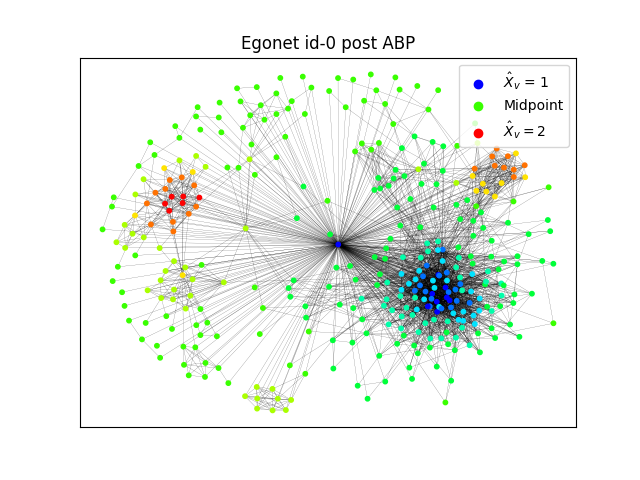
\includegraphics[width=\figwidth]{ego-0-abp.png}
	\caption{Normalised ABP output $\tilde{\sigma}_v$ colouring vertices, spring layout}
	\label{fig:abp-output-norm}
\end{figure}

We colour each vertex according to this quantity $\tilde{\sigma}_v$ and plot the graph
\footnote{ABP is non-deterministic so each figure is the result of a different run of ABP. No exact comparison is possible between figures but the results are in some sense typical.}
on figure \ref{fig:abp-output-norm}. We see intuitively that ABP has worked. The blue cluster in the lower right is clearly part of the same community. Furthermore, many vertices that do not seem to belong to any cluster have uncertain classifications (the colour is close to green). Inspecting figure \ref{fig:ego-0-by-gender} shows us that the sets $S$ and $S^C$ do separate nicely with high intra-group connectivity and lower inter-group connection density. After all, we seek to find a roughly balanced partition that minimises the number of edges between the two sets.
%
\begin{figure}[H]
	\centering
	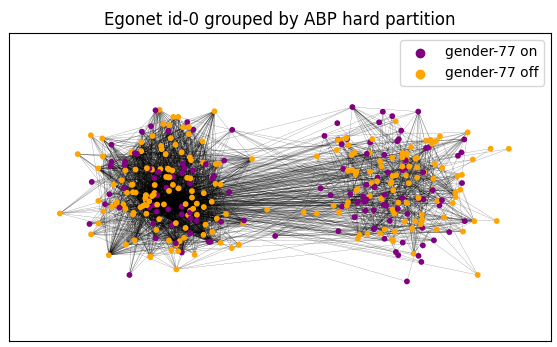
\includegraphics[width=\figwidth]{ego-0-abp-by-gender.png}
	\caption{Vertices grouped by ABP partition: set $S$ (left cluster) and set $S^C$ (right cluster)}
	\label{fig:abp-output-by-gender}
\end{figure}

Within set $S$ we have $\{58, 122\}$ 77-ers and 78-ers respectively and for $S^C$ the breakdown is $\{72, 96\}$. Therefore, the fraction of each gender cohort in set S can be calculated:
%
\begin{equation}
	\begin{aligned}
	\frac{|\Omega_{77} \cap S|}{|\Omega_{77}|} &= \frac{58}{58+72} = 0.446 \\
	\frac{|\Omega_{78} \cap S|}{|\Omega_{78}|} &= \frac{122}{122+96} = 0.560
	\end{aligned}
\end{equation}
%
Clearly the fractions of each community in the partition $S$ differ substantially so we say that weak recovery is solved. The set $S$ contains a higher proportion of the overall 78-population than of the 77-population.

\subsection{From detection to inference}
\label{sect:detection-to-inference}

We now have an algorithm (ABP) that partitions our graph into two sets that are maximally distinct from a clustering sense. We can now ask the question of which vertex labels most readily explain the separation. Therefore, we can determine which features have the largest impact on the graphical structure; this circumvents the binary resolution problem with the hypothesis testing approach.

This part of the project is still in its early stages so these are just preliminary results. We necessarily remove the constraint on the community sets $\Omega_i$ to be disjoint as one vertex can have multiple features turned on. We perform a linear regression on the $n \times 1$ normalised belief vector $\tilde{\sigma}$ with the $n \times f$ feature matrix $F$ as the explanatory variable. $F_{ij} = 1$ if vertex $i$ has feature $j$ turned on and $0$ if feature $j$ is off. The equation we try to fit is given below:
%
\begin{equation}
	\tilde{\sigma} = a + F b + \epsilon
	\label{eqn:lin-regression}
\end{equation}
%
Linear regression finds the constant bias $a$ and $f \times 1$ weight vector $b$ that minimises the mean squared prediction error $\epsilon^T \epsilon / n$. The theory for linear regression is well known so omitted here (see \cite{yale-linear-regression} for a reference). We restrict $F$ to only include gender and language features and plot the regression coefficient for each feature in order of decreasing magnitude (figure \ref{fig:abp-output-lin-regression}).
%
\begin{figure}[H]
	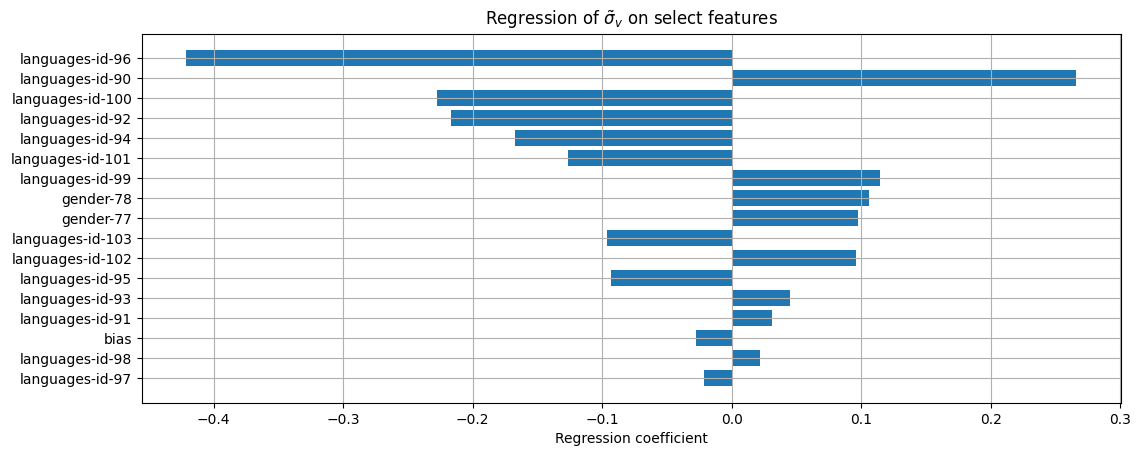
\includegraphics[width=\linewidth]{ego-0-abp-lin-regression.png}
	\caption{Egonet-0 linear regression of $\tilde{\sigma}_v$ on select features ($R^2 = 0.113$)}
	\label{fig:abp-output-lin-regression}
\end{figure}

The results are rather interesting. Certain languages are a far stronger predictor of community assignment than gender. After all, one would hope that a language barrier poses a more tangible obstacle to friendship than gender. The bias term has rather low magnitude which just implies that the partition $S$ and $S^C$ are of similar size.

This analysis is of course rather crude as we have failed to take into account multi-collinearity or even determined if a linear regression model is appropriate; indeed, an $R^2$ value of just 0.113 would suggest that it is not. Nevertheless, this serves as the platform for subsequent more rigorous analysis. Furthermore, we have not yet proven the conjecture that the regression coefficients are valid measures of causal impact on graphical structure.

\section{Future Direction}

The immediate next steps for the project are to refine the classification approach outlined in section \ref{sect:detection-to-inference}. Firstly, it should be tied back to the hypothesis testing framework to make sure that the results are proven to be meaningful. Secondly, the exact form of the classifier can be explored; a linear regression model is a good starting point but we can expand to a softmax neural network as that would allow us to generalise to more than just two partitions.

Indeed, ABP is severely limited by the fact that it only outputs 2 sets. Though weak recovery is solved, the partition is often hard to interpret as various clusters get subsumed into one. We instead would prefer to investigate algorithms that can identify arbitrarily many clusters. Force-directed approaches are the standard in industry for their speed of execution. One of the most common is the Fruchterman-Reingold algorithm which treats vertices as repelling objects and edges as restoring forces. It can then perform iterative updates on vertex positions until convergence or termination. This algorithm is what is used by the NetworkX package \cite{networkx} to compute graph layouts as seen in figures \ref{fig:ego-0-by-gender} and \ref{fig:abp-output-norm}. Song and Bressan \cite{force-directed} have had great success using the Fruchterman-Reingold algorithm followed by k-means clustering for community detection.

Lastly, the analysis must of course be expanded to more datasets to benchmark efficacy against existing methods and ensure the approach is generally applicable. Work has already begun analysing the influence of gender on academic collaboration graphs provided by Aminer \cite{aminer}. Nevertheless, this dataset does not contain gender explicitly, only first-name. However, this is cross-referenced with a list of popular baby-names to get a good replacement (as suggested by West et al. \cite{gender-scholarship}). Furthermore, the seminal dataset of political blogs from the 2004 US election \cite{polblogs} which started much of the analysis of the SBM will of course be analysed.

\section{Conclusion}

This concludes the Technical Milestone Report for the project thus far. We start by fully fleshing out the theoretical foundation of the Stochastic Block Model and hypothesis tests on connectivity parameters. Nevertheless, this approach is too narrow in scope to be a useful tool on its own. We therefore set about the problem from the opposite direction; rather than verify structure we are already given, we detect structure in the graph without using labels and seek to identify which labels best recreate the detected partition. Early results are promising but this approach needs to be given the same rigorous treatment as the hypothesis testing framework. That will be the emphasis of future work.

\printbibliography

\end{multicols*}

\end{document}
